\documentclass[border=4pt]{standalone}
% Paleta y fuentes compartidas por el libro y las figuras (única fuente de verdad).
\RequirePackage{xcolor}
\definecolor{oxido}{HTML}{B7410E}
\definecolor{cobre}{HTML}{D27D2D}
\definecolor{carbon}{HTML}{2B2B2B}
\definecolor{azul}{HTML}{1F5F8B}
\definecolor{arena}{HTML}{F4EDE4}

\usepackage{fontspec,pgfplots}
\pgfplotsset{compat=1.18}
\pgfkeys{/pgf/number format/assume math mode=true,/pgf/number format/use comma}
\setsansfont{FiraSans}[Extension=.otf,UprightFont=*-Regular,BoldFont=*-SemiBold,ItalicFont=*-Italic]
\begin{document}
\sffamily\small
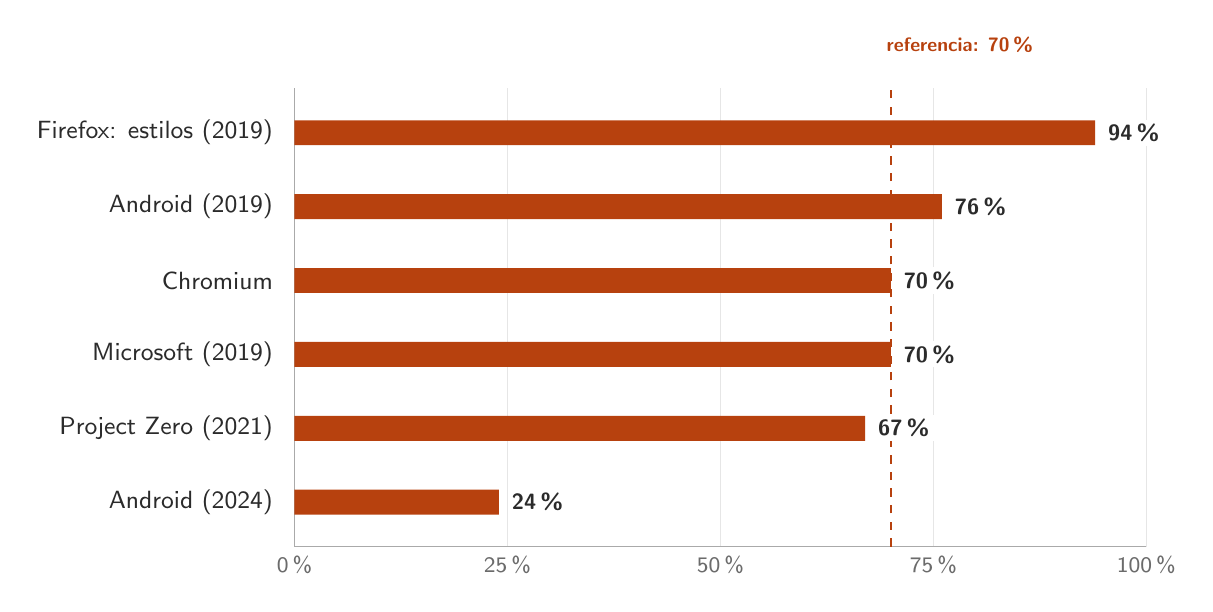
\begin{tikzpicture}
\begin{axis}[
  xbar, width=12.4cm, height=7.4cm,
  xmin=0, xmax=100, bar width=9pt,
  symbolic y coords={Android 2024,Project Zero 2021,Microsoft 2019,Chromium,Android 2019,Firefox estilos 2019},
  ytick=data,
  yticklabels={Android (2024),Project Zero (2021),Microsoft (2019),Chromium,Android (2019),Firefox: estilos (2019)},
  y tick label style={font=\sffamily\small,text=carbon},
  xtick={0,25,50,75,100}, xticklabel={\pgfmathprintnumber{\tick}\,\%},
  x tick label style={font=\sffamily\footnotesize,text=carbon!70},
  axis x line*=bottom, axis y line*=left,
  xmajorgrids, grid style={carbon!12},
  axis line style={carbon!40}, tick style={draw=none},
  enlarge y limits=0.12,
  nodes near coords={\pgfmathprintnumber{\pgfplotspointmeta}\,\%},
  nodes near coords style={font=\sffamily\footnotesize\bfseries,text=carbon,anchor=west,xshift=3pt,fill=white,inner sep=1.5pt},
  point meta=x,
  extra x ticks={70}, extra x tick labels={},
  extra x tick style={grid=major, major grid style={oxido,dashed,thick}},
]
\addplot[fill=oxido,draw=none] coordinates {
  (24,Android 2024) (67,Project Zero 2021) (70,Microsoft 2019)
  (70,Chromium) (76,Android 2019) (94,Firefox estilos 2019)};
\end{axis}
\node[font=\sffamily\scriptsize\bfseries,text=oxido,anchor=south] at (8.45,6.15) {referencia: 70\,\%};
\end{tikzpicture}
\end{document}
